\section{Durchführung}
\label{sec:Durchführung}

In der folgenden Abbildung \ref{fig:Aufbau} ist der Aufbau zunächst schematisch
dargestellt. Der Cantilever-Arm ist auf die Probe gerichtet und seine
Auslenkung wird mittels eines Lasers ($\SI{635}{\nano\meter}$) ermittelt. Der
am Cantilever-Rücken reflektierte Laserstrahl wird von einem
Viersegment-Photodetektor registriert, sodass die Auslenkung anhand der
registrierten Intensität bestimmt werden kann (siehe Unterkapitel
\ref{sec:Rasterkraftmikroskop}). Der Detektorstrom wird an einen PC weitergeben
und dort ausgewertet. Unterschiedliche Verfahren erlauben es, die Probe abzurastern.
In diesem Versuch ist die Cantilever-Apparatur fest montiert. Hingegen wird die
Probe mittels piezo-elektrischen Elementen in alle drei Raumrichtungen bewegt.
Zur Ansteuerung dienen jeweils drei Piezo-Controller. Im Folgendem wird der
piezo-elektrische Effekt genauer erklärt.

\begin{figure}[H]
	\centering
	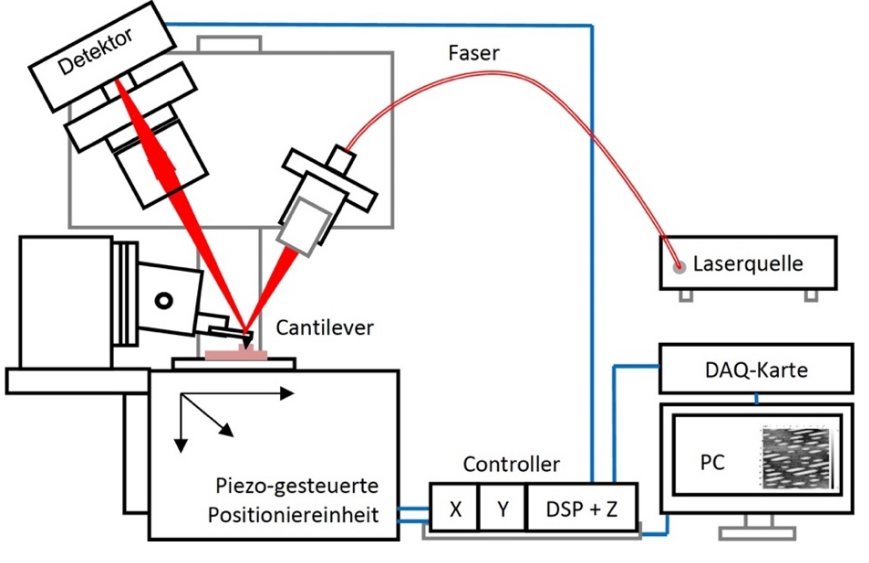
\includegraphics[width=0.8\textwidth]{Abb/Aufbau.png}
	\caption{Schematische Darstellung des Versuchsaufbaus	\cite[2]{anleitung}.}
	\label{fig:Aufbau}
\end{figure}

\noindent
Der piezo-elektrische
Effekt tritt nur bei Kristallen wie Silizium auf, da diese kein Inversionszentrum
aufweisen. Nur dann heben sich die Oberflächenladungen in der Polarisationsrichtung
nicht mehr auf, sodass sich in Anwesenheit eines externen E-Feldes der Kristall
ausdehnt/zusammenzieht. Verantwortlich für die Kristallvolumenänderung ist ein
intrinsischer Effekt, welcher allerdings stets von einem unerwünschten extrinsischen
Effekt begleitet wird. Der intrinsische Effekt
verschiebt dabei die Kristall-Ionen bei Anwesenheit eines externen E-Feldes, sodass sich
dies makroskopisch als Kristallvolumenänderung bemerkbar macht. Dieser Effekt ist
annähernd linear und zeigt keine Hysterese. Der extrinsische Effekt ist für die
Neuorientierung der ferroelektrischen Domänen verantwortlich und unterliegt damit der Hysterese.
Angenommen die Dipolmomente haben sechs Orientierungsmöglichkeiten
und der Kristall damit sechs unterschiedliche Typen von Domänen. Wird das E-Feld nun in
die Polarisationsrichtung angelegt, können sich die Dipolmomente, nach Überwindung
einer Energiebarriere, (anti-)parallel zum E-Feld ausrichten. Vier der Domänen
schrumpfen, während die zwei übrigen Domänen größer werden. Wie lange es dauert,
bis sich die Dipolmomente entlang des E-Feldes ausrichten und der Kristall sich damit
ausdehnt/zusammenzieht, hängt also von seiner Vorgeschichte ab. Zusammengefasst
hängt die Antwort des Kristall-Systems von seinem inneren Zustand ab. Dieses
Verhalten ist in Abbildung \ref{fig:butterfly} der Einfachheit halber für zwei
Orientierungen dargestellt. Am Punkt 1 ist das E-Feld stark genug, sodass alle
Dipolmomente parallel ausgerichtet sind. Wird das E-Feld abgeschaltet, so
richten sich einige Dipolmomente antiparallel aus. Dennoch überwiegen die parallel
ausgerichteten Dipolorientierungen. Zwischen diesen beiden Punkten überwiegt der
erwünschte intrinsische Effekt.
Nun wird das E-Feld in umgekehrter Richtung eingeschaltet und die Netto-Polarisation
wird am Punkt 3 gleich Null. Mit stärker werdendem E-Feld richten sich am Punkt 4 alle
Dipolmomente antiprallel aus. Am Punkt 5 ist das E-Feld wieder abgeschaltet und
die Minderheit der Dipolmomente hat sich wieder in paralleler Richtung orientiert.
Zuletzt wird das E-Feld ein weiteres Mal umgekehrt und es ergibt sich bei Punkt 6
wieder eine Netto-Polarisation
von Null. Im Verlauf von Punkt 3 nach 6 haben sich die Domänen vollständig neu orientiert,
sodass der unerwünschte extrinsische Effekt teilweise dominiert hat. Um Hysterese
zu vermeiden, sollte das piezo-elektrische Element zwischen den Punkte 1-2 betrieben
werden. Zusätzlich kommen Dehnungssensoren, die sogenannten $\textit{Strain Gauges}$,
zum Einsatz, welche diesem Problem entgegenwirken.


\begin{figure}[H]
	\centering
	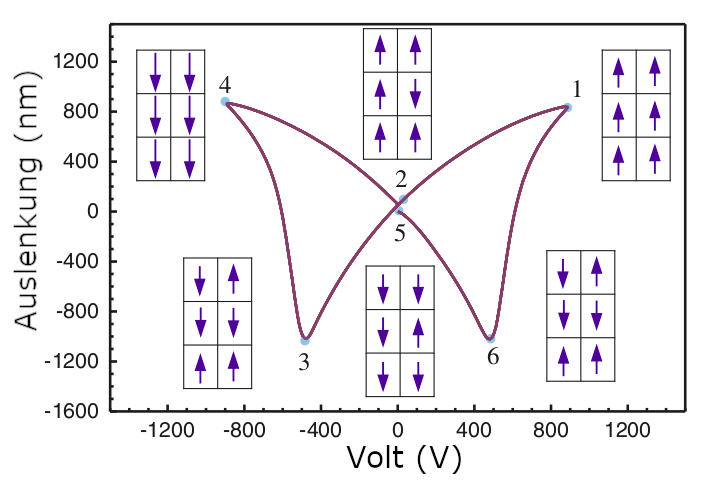
\includegraphics[width=0.63\textwidth]{Abb/butterfly.png}
	\caption{Schematische Darstellung des schmetterlingsförmigen Verhaltens der
	ferroelektrischen Domänen eines piezo-elektrischen Elements. Im Bereich zwischen
	den Punkten 1 und 2 überwiegt	der intrinsische Effekt. In den darauffolgenden
	Punkten dominiert der extrinsische Effekt teilweise. Das piezo-elektrische
	Element sollte damit nur in dem Bereich zwischen dne Punkten 1 und 2 arbeiten
	\cite[47]{AFM}.}
	\label{fig:butterfly}
\end{figure}

\noindent
In diesem Versuch wird ausschließlich im $\textit{Constant-Force}$-Modus gemessen.
Um die Kraft bzw. die Auslenkung konstant halten zu können, wird dem Piezo-Controller
in z-Richtung ein digitaler Signalprozessor (DSP) vorgeschaltet. Dieser verarbeitet
die über die Viersegment-Photodiode registrierte Auslenkung und gibt dem Piezo-Controller
ein Feedback-Signal wieder. Die z-Position der Probe wird dann mittels der
Photodioden-Controller$\&$Auto-Aligner so nachgeregelt, dass die Auslenkung
konstant bleibt.\\
Um die Topografie einer Probe untersuchen zu können, wird die Messspitze mit Hilfe
einer Kamera auf die Probe geführt. Sobald Messspitze und Probe in Kontakt stehen,
kann eine z-Piezospannung gemessen werden. Der optimale Messbereich liegt
zwischen 0-$\SI{50}{\volt}$, sodass die Höhe der Messspitze auf eine
z-Piezospannung von $\SI{25}{\volt}$ eingestellt wird. Zunächst wird eine
Siliziumdioxid-Mikrostrukturprobe (siehe Abbildung \ref{fig:MSP}) untersucht.

\begin{figure}[H]
	\centering
	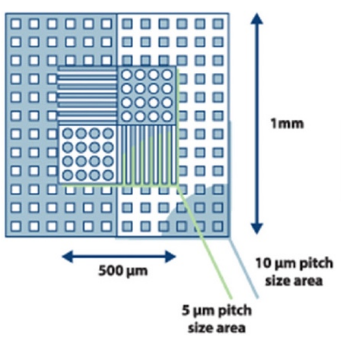
\includegraphics[width=0.5\textwidth]{Abb/MSP.png}
	\caption{Schematische Darstellung der Mikrostrukturprobe. Dabei handelt es sich
	um einen Silizium-Sockel mit $\SI{100}{\nano\meter}$ dicken Siliziumdioxid-Schichten,
	welche die Mikrostrukturen bilden	\cite[4]{anleitung}.}
	\label{fig:MSP}
\end{figure}

\noindent
Dann wird die Topografie unterschiedlicher Speichermedien (CD, DVD, Blu-ray)
untersucht und daraus die maximale Speicherkapazität der CD bestimmt.
Die bei der Topografie-Messung verwendeten Einstellungen sind in Tabelle \ref{tab:einst}
ersichtlich.


\begin{table}
  \centering
  \caption{Einstellungen zu den Topografie-Messungen}
  \label{tab:einst}
  \sisetup{table-format=1.2}
  \begin{tabular}{S S S S}
    \toprule
    {Probe} & {Scanfenster} & {Scanparameter} & {Scangeschwindigkeit} \\
		{} & {$\SI{}{\micro\metre\squared}$} & {Pixel$^2$} & {Pixel/s} \\
    \midrule
    {Mikrostruktur} & {20x20} & {250x250} & {100} \\
		{CD}						& {10x10} & {250x250} & {100} \\
		{DVD}						& {5x5}   & {250x250} & {100} \\
		{Blu-ray}			& {2x2}	  & {250x250} & {50}  \\
    \bottomrule
  \end{tabular}
\end{table}

\noindent
Abschließend wird die z-Nachreglung deaktiviert und eine z-Piezospannung von
$\SI{8}{\volt}$ eingestellt, um eine Kraft-Abstandkurve von Edelstahl, Teflon
und einer TiN-Schicht aufzunehmen.
